\section{Introducción}
\subsection*{Antecedentes y motivación}

\begin{frame}{Introducción}{Antecedentes y motivación}
Web 2.0
\begin{itemize}
\item Grandes cantidades de datos
\item Cómo procesar esta información en tiempo real
\end{itemize}

\begin{figure}
  \center
    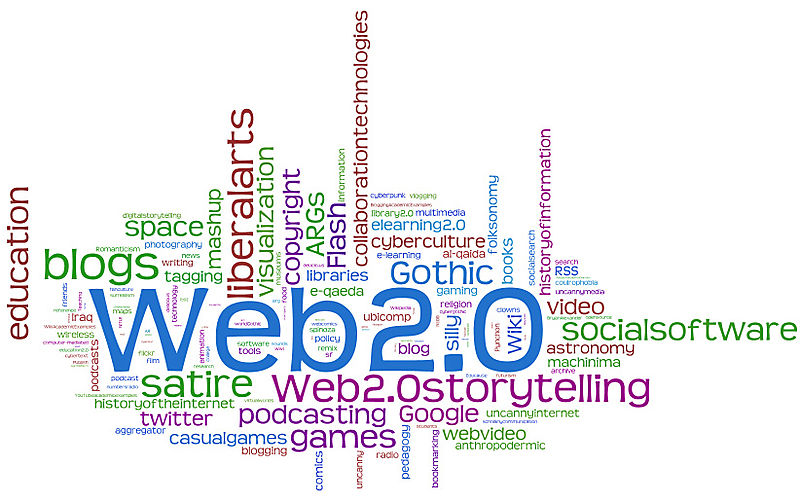
\includegraphics[scale=0.35]{images/Web.jpg}
\end{figure}
\end{frame}

\begin{frame}{Introducción}{Antecedentes y motivación}
\begin{itemize}
\item Superar restricciones de temporalidad
\item Manejo de grandes flujos de datos en tiempo real
\item Respuestas rápidas y actualizadas
\item Apoyo en la toma de decisiones
\end{itemize}
Por ejemplo:
\begin{itemize}
	%\item Análisis de sentimientos de los mensajes de usuarios 
	\item Predicciones del comportamiento en la \textbf{bolsa de valores}
	\item Recopilación de información en \textbf{caso de emergencia}
	\item Monitoreo de registros para la \textbf{seguridad en redes}
\end{itemize}
\end{frame}

\begin{frame}{Introducción}{Antecedentes y motivación}
\begin{itemize}
\item Tipos de sistemas de procesamiento de \textsl{stream}
	\begin{itemize}
	\item S4
	\item Storm
	\item Samza
	\end{itemize}
\item \textsl{Problemas}
	\begin{itemize}
	\item Poca adaptaci\'on del sistema en tiempo de ejecución
	\item Posibles problemas de distribución de carga
	\item Baja en el rendimiento
	\item Pérdida de recursos e información
	\end{itemize}
\end{itemize}
\end{frame}

%\subsection*{Descripción del problema}
%
%\begin{frame}{Introducción}{Descripción del problema}
%\begin{block}{}
%	Dado el carácter estático del grafo de procesamiento en tiempo de ejecución y el carácter altamente dinámico del tráfico, pueden surgir problemas de balance de carga entre los operadores de la topología, sobrecargando alguno de estos y comprometiendo el rendimiento del sistema.
%\end{block}
%\end{frame}